\documentclass[12pt]{article}

\usepackage{geometry}
\geometry{top=1.5cm,bottom=3cm,left=1.2cm,right=2cm}


\usepackage{array}
\usepackage{color}
\usepackage{graphicx}
\usepackage{fancyhdr}
\usepackage[UTF8]{inputenc}
\usepackage[spanish]{babel}
\usepackage{t1enc}
\usepackage{fontsmpl}
%\usepackage{titlesec}
\usepackage{enumerate}
\usepackage{enumitem}

\usepackage{subcaption}
\usepackage{float}

\usepackage{listings,xcolor,bm}


\definecolor{mygreen}{rgb}{0,0.6,0}
\definecolor{mygray}{rgb}{0.5,0.5,0.5}
\definecolor{mymauve}{rgb}{0.58,0,0.82}
\lstset{
  backgroundcolor=\color{white},   % choose the background color; you must add
  basicstyle=\ttfamily,      % the size of the fonts that are used for the code
  breakatwhitespace=true,         % sets if automatic breaks should only happen at whitespace
  breaklines=true,                 % sets automatic line breaking
  captionpos=b,                    % sets the caption-position to bottom
  commentstyle=\color{mygreen},    % comment style
  deletekeywords={...},            % if you want to delete keywords from the given language
  escapeinside={\%*}{*)},          % if you want to add LaTeX within your code
  extendedchars=true,              % lets you use non-ASCII characters; for 8-bits encodings only, does not work with UTF-8
  firstnumber=1,                % start line enumeration with line 1000
  frame=single,	                   % adds a frame around the code
  keepspaces=true,                 % keeps spaces in text, useful for keeping indentation of code (possibly needs columns=flexible)
  keywordstyle=\color{blue},       % keyword style
  language=Python,                 % the language of the code
  morekeywords={*,...},            % if you want to add more keywords to the set
  numbers=none,                    % where to put the line-numbers; possible values are (none, left, right)
  numbersep=5pt,                   % how far the line-numbers are from the code
  numberstyle=\tiny\color{mygray}, % the style that is used for the line-numbers
  rulecolor=\color{black},         % if not set, the frame-color may be changed on line-breaks within not-black text (e.g. comments (green here))
  showspaces=false,                % show spaces everywhere adding particular underscores; it overrides 'showstringspaces'
  showstringspaces=false,          % underline spaces within strings only
  showtabs=false,                  % show tabs within strings adding particular underscores
  stepnumber=5,                    % the step between two line-numbers. If it's 1, each line will be numbered
  stringstyle=\color{mymauve},     % string literal style
  tabsize=4,	                   % sets default tabsize to 2 spaces
  title=\lstname,                  % show the filename of files included with \lstinputlisting; also try caption instead of title
  belowskip=0em
}

\usepackage{multicol}
\def\RR{{\rm I}\!\!{\rm R}}
\def\NN{{\rm I}\!{\rm N}}
\def\ZZ{{\rm Z}\!\!{\rm Z}}
\def\di{\displaystyle}

\def\sen{\mbox{sen\,}}

\newcommand{\encabezado}[1]
{

\noindent\usefont{T1}{phv}{m}{n}
{Matem\'atica 2 (B)\\
Segundo Cuatrimestre - 2020}\\
\smallskip

\noindent{\large Pr\'actica 6: An\'alisis de datos}\\[-0.2cm]
\hrule
\normalfont}

%\setlength{\parskip}{\baselineskip}

\setlength{\parindent}{0pt}
\renewcommand{\labelenumiii}{\roman{enumiii}) }


\begin{document}

\centerline{{\small Universidad de Buenos Aires - Facultad de Ciencias Exactas y Naturales - Ciencias de Datos}}

\vskip 0.2cm

\hrule

\vskip 0.2cm

 \centerline{{\bf\Large{\sc Laboratorio de Datos}}}

 \vskip 0.2cm

 \centerline{\ttfamily Primer Cuatrimestre 2024}

\vskip 0.2cm

 \hrule

 \bigskip
 \centerline{\bf Simulacro Parcial}
 \bigskip


\thispagestyle{plain}


%\renewcommand{\labelenumi}{\textbf{Ejercicio} \theenumi.}


%%--------------------------------------
%
%\item Implementar un programa que reciba como input un archivo de texto \textit{archivo.txt} y devuelva los coeficientes de la regresi\'on lineal de las componentes principales de \textit{archivo.txt}.
%
%\setlength{\parskip}{\baselineskip}
%


%----------------------------------------------------------
% 1


\begin{enumerate}

\item Se quiere estimar el nivel de colesterol en sangre por regresión lineal utilizando los siguientes datos de los pacientes: índice de masa corporal, minutos de ejercicio físico diario, cantidad de grasas ingeridas por día. Si se agrega una nueva variable ``último dígito del DNI del paciente'', y se compara con el modelo anterior mediante un esquema de entrenamiento y testeo, como espera que se modifique el error cuadrático medio (ECM):
    
\begin{enumerate}
\item Aumenta el ECM tanto en entrenamiento como en testeo.
\item Aumenta el ECM en entrenamiento y disminuye en testeo.
\item Disminuye el ECM en entrenamiento y aumenta en testeo.
\item Disminuye el ECM en entrenamiento y testeo.
\end{enumerate}

%\item Para el siguiente DataFrame, ¿cuál es el resultado de aplicar el siguiente comando?
%
%\begin{table}[h!]
%    \centering
%    \begin{tabular}{|c|c|c|}
%        \hline
%        \textbf{Patas} & \textbf{Animal} & \textbf{Reino} \\
%        \hline
%        0 & Pez Dorado & Peces \\
%        \hline
%        2 & Gorrión & Aves \\
%        \hline
%        4 & Perro & Mamíferos \\
%        \hline
%        6 & Hormiga & Insectos \\
%        \hline
%        2 & Pingüino & Aves \\
%        \hline
%        4 & Gato & Mamíferos \\
%        \hline
%        0 & Tiburón & Peces \\
%        \hline
%        4 & Vaca & Mamíferos \\
%        \hline
%        2 & Paloma & Aves \\
%        \hline
%    \end{tabular}
%    \caption{Conjunto de datos sintéticos con el número de patas, nombres de animales y su correspondiente reino animal}
%    \label{tab:legs_animal_kingdom}
%\end{table}
%
%
%\begin{lstlisting}
%df.groupby("reino")["patas"].mode()
%\end{lstlisting}

\item ¿Cuál de los siguientes comandos de Python calcula correctamente el error cuadrático medio entre el vector respuesta y el vector de predicciones?
\begin{enumerate}
\item \lstinline{np.sum((y - y_pred)**2) / len(y)}
\item \lstinline{np.sum((y - y_pred))**2 / len(y)}
\item \lstinline{(y.mean())**2 - (y_pred.mean())**2)}
\item \lstinline{np.mean(pd.concat([y, y_pred])**2)}
\end{enumerate}
%\begin{lstlisting}
%df.groupby("species")["sex"].values_count()
%\end{lstlisting}

\item Decidir V o F.

\begin{enumerate}
\item Ambos métodos de clustering $k$-medias y DBSCAN son sensibles a la escala de los datos.
\item Como medida de centralidad de datos, la mediana es menos sensible a outliers que la media.
\item Clustering es un problema de aprendizaje supervisado.
\item KNN es un método de clasificación no parámetrico.
\item Regresión lineal es un método de aprendizaje supervisado y regresión Ridge es un método de aprendizaje no supervisado.
\end{enumerate}

\item 
En la siguiente tabla se muestran las edades de los pacientes que recibió un médico un día. Se realiza un boxplot para resumir los datos (utilizando bigotes de longitud hasta 1.5 veces la distancia intercuartil). ¿Cuál de los cuatro box-plot es el correcto?

\item 
\begin{table}[h!]
    \centering
    \begin{tabular}{|*{10}{c|}}
        \hline
        \textbf{Index} & 1 & 2 & 3 & 4 & 5 & 6 & 7 & 8 & 9\\
        \hline
        \textbf{Edad} & 12 & 15 & 27 & 35 & 37 & 40 & 45 & 50 & 84 \\
        \hline
    \end{tabular}
    \caption{Table of ages in one row}
    \label{tab:ages}
\end{table}


\begin{figure}[H]
    \centering
    \begin{subfigure}[b]{0.45\textwidth}
        \centering
        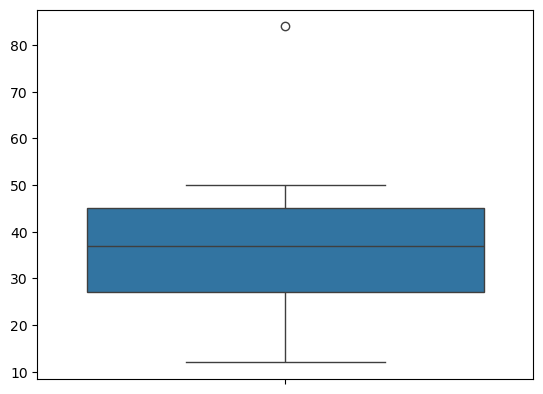
\includegraphics[width=\textwidth]{simu-boxplot1.png}
        \caption{Image 1}
        \label{fig:image1}
    \end{subfigure}
    \hfill
    \begin{subfigure}[b]{0.45\textwidth}
        \centering
        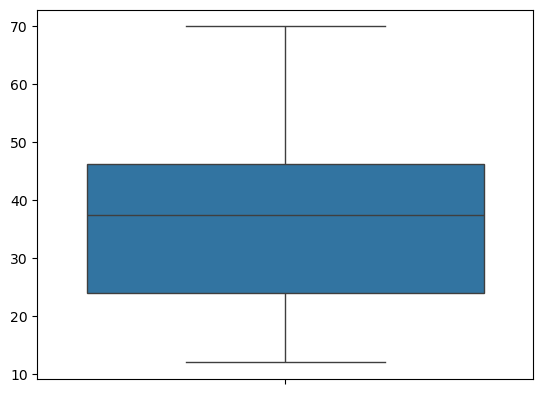
\includegraphics[width=\textwidth]{simu-boxplot2.png}
        \caption{Image 2}
        \label{fig:image2}
    \end{subfigure}
    \vskip\baselineskip
    \begin{subfigure}[b]{0.45\textwidth}
        \centering
        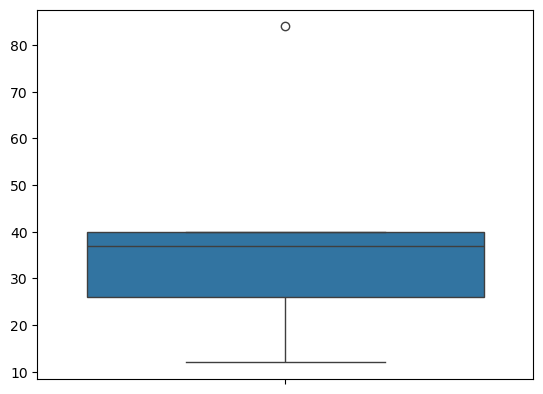
\includegraphics[width=\textwidth]{simu-boxplot3.png}
        \caption{Image 3}
        \label{fig:image3}
    \end{subfigure}
    \hfill
    \begin{subfigure}[b]{0.45\textwidth}
        \centering
        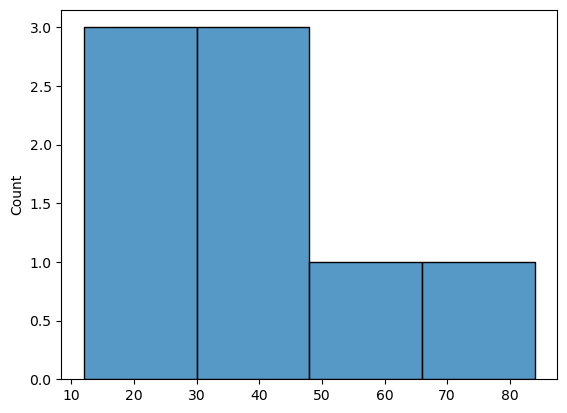
\includegraphics[width=\textwidth]{simu-boxplot4.png}
        \caption{Image 4}
        \label{fig:image4}
    \end{subfigure}
    \caption{Four images arranged in two columns.}
    \label{fig:four_images}
\end{figure}
    
\item Se quiere realizar un clustering con estos datos. ¿Cuál de las siguientes opciones considera que es la más apropiada?

\begin{enumerate}
\item $k$-medias con $k = 2$
\item $k$-medias con $k = 3$
\item DBSCAN con $\varepsilon = 0.2$ y $minPts = 20$
\item DBSCAN con $\varepsilon = 0.5$ y $minPts = 20$
\end{enumerate}

\item Completar el codigo falta para cada uno de los siguientes gráficos.

\begin{enumerate}
\item 
\begin{lstlisting}
(
    so.Plot(data = penguins, x = "bill_length_mm", y = "bill_depth_mm", ???)
    .add(so.Line(), so.PolyFit(1))
)
\end{lstlisting}
\item 
\begin{lstlisting}
(
    so.Plot(data = penguins, ???)
    .add(so.Bars(), so.Hist())
)
\end{lstlisting}
\item 
\begin{lstlisting}
(
    so.Plot(???)
    .add(so.Bars(), so.Hist())
)
\end{lstlisting}
\item 
\begin{lstlisting}
(
    so.Plot(data = gapminder, ???)
    .add(so.Line())
)
\end{lstlisting}

\end{enumerate}

\item Para el siguiente conjunto de datos, aplicar en Python alguna técnica de clustering para obtener clusters como los de la figura de la derecha
    
\item Para el conjunto de datos en el archivo \lstinline{datos.csv}, calcular:
\begin{enumerate}
\item El promedio de la variable ``altura''.
\item El peso medio para 
\end{enumerate}

\end{enumerate}

\end{document}
